\documentclass{article}
\usepackage[utf8]{inputenc}
\usepackage{listings}
\usepackage{siunitx}
\usepackage{graphicx}
\usepackage{float}
\usepackage{color}
\usepackage[toc,page]{appendix}

% Add a micro symbol that we use once
\sisetup{math-micro=\text{µ},text-micro=µ}

%%%% BEGIN XML LISTINGS %%%%
\usepackage{color}
\definecolor{gray}{rgb}{0.4,0.4,0.4}
\definecolor{darkblue}{rgb}{0.0,0.0,0.6}
\definecolor{cyan}{rgb}{0.0,0.6,0.6}

\lstset{
  basicstyle=\ttfamily,
  columns=fullflexible,
  showstringspaces=false,https://www.overleaf.com/1335294559stbjrgndybkm
  commentstyle=\color{gray}\upshape
  }

\lstdefinelanguage{XML}
{
  morestring=[b]",
  morestring=[s]{>}{<},
  morecomment=[s]{<?}{?>},
  stringstyle=\color{black},
  identifierstyle=\color{darkblue},
  keywordstyle=\color{cyan},
  morekeywords={xmlns,version,type}% list your attributes here
}
%%%% END XML LISTINGS %%%%

\title{Analysis}
\author{Bram het Wit, Maurizio Giannattasio \& Stefan Schokker}
\date{January 2020}

\begin{document}

\begin{titlepage}
	\maketitle
\end{titlepage}

\begin{abstract}
    In this paper we will discuss our process, our findings and discuss some further improvements. 
\end{abstract}

\tableofcontents
\listoffigures

\newpage

\section{Research Questions}
\subsection{Beginning of the project}
At the start of the project we had a fairly broad research question in mind. Namely "What methods could be used to increase energy efficiency in scientific research?". As time went on, we began to understand that we couldn't use the existing setup to gather accurate data. This meant that the majority of our project wasn't aimed at processing data and doing tests, but building a better testing environment. In our opinion this worked out quite alright, with only a few points left for further improvement, given the data that we want to collect.
\subsection{A more realistic research question}
So we ended up narrowing our main research question to "How to build an efficient an relatively easy to use power monitor to use in a super computer simulation". While this is a really specific question, we still took nearly the entire semester to answer it. Our most important sub question, "What kind of workload do we want to simulate that's worth measuring" also took a lot of time to fill in. After we would have figured that out, we we had to find out what the most effective way to monitor and collect our data would be, and how to visualise that data. To find out what we wanted to simulate we made sure to look at what algorithms are regularly used in radio astronomy, and how they are used.

% What methods could be used to increase energy efficiency in scientific research?

%     -What are the most efficient ways to monitor power consumption 
%         -How are we going to monitor it?
%         -How are we going to visualise it? 

%     -What are the best platforms to use in our testing environment?

%     -What is the best way to simulate scientific research in our testing environment?
%         -What algorithm or program will we run on our 
%                          platforms to test the power consumption?    


\section{Algorithm tests}

For our final tests we had two algorithms prepared. A Mandelbrot using MPI and a FFT using MPI. The basic idea of the raspberry pi stack is simulating a supercomputer dealing with astronomical data. We use MPI for multiprocessing and the algorithms have been chosen on the basis that they are comparable to the processes performed by supercomputers in dealing with astronomical data.

The way we chose the algorithm and how it works is described in more detail in the algorithm paper.

\subsection{FFT algorithm}

There are two tests that use the FFT algorithm, the FFT\_with\_MPI test and the FFT\_with\_multithreading test.\par The FFT with multi threading test does a two dimensional Fourier transform over an image, and transforms it back as well. It generates three bitmaps, one to see how the program interprets the input, one to see how the image looks like in the Fourier domain, and the last one is the inverse Fourier transformed image back to the normal image to see if the program didn't mess up the data. This program can be run on a single pi and the amount of threads used can be set.\\

The other test that uses the FFT library uses MPI, this test however does not take an image as input. It only fills an array with some data and then preforms a Fourier transform by dividing the load over all the machines it has avalible via MPI. 

\subsection{Mandelbrot algorithm}
The mandelbrot algorithm was chosen because it provided a load big enough to get interesting results. While the FFT is a more interesting choice for radio astronomy, the programs are not quite yet capable of interpreting a big input. The mandelbrot test makes the pi's calculate a 4096 by 4096 mandelbrot image which can take up to several minutes, and is therefore a more accurate representation of a real heavy load than the FFT programs. If the FFT programs are fixed to interpret bigger inputs the mandelbrot algorithm might not be needed anymore.   

\subsection{Running tests}
The run the test all raspberry pi's need to have open MPI installed on them. One raspberry pi is made the host. This raspberry pi will start the algorithm and tell the other raspberry pi's what they need to do. To start a program the following command is used "mpiexec -n 'amount of processes' -machinefile machinefile ./'the program'". Depending on the amount of processes the host pi will activate cores on different raspberry pi's to perform calculations. Every raspberry pi has four cores to be used, the order the cores on the raspberry pi's are used is specified in a machine file in which the addresses of the different raspberry pi's are listed. 
\newline
We ran our test with a increasing number of cores. The starting time was noted for each run. When the program closed we noted the end time and filled the calculated run-time from the programs in separately. The run-time only kept track of the start and end of the MPI, to accurately calculate the power consumption we separately kept of the opening and closing of the program. This could be automated see chapter Future plans. The run-time was used to calculate the kWh consumption for the algorithm. The calculation of the average power used during a run is being done with a python script. This script can be further develop to speed up the analysis of results, see chapter Future plans for more information. 
\newline
In figure\ref{fig:Mandelgnuplot} and \ref{fig:FFTgnuplot} the power used by the raspberry pi's during a Mandelbrot and FFT test are plotted. The Mandelbrot started with two cores while the FFT started with one core. The Mandelbrot was unable to function with only one core.

\begin{figure}[H]
\centering
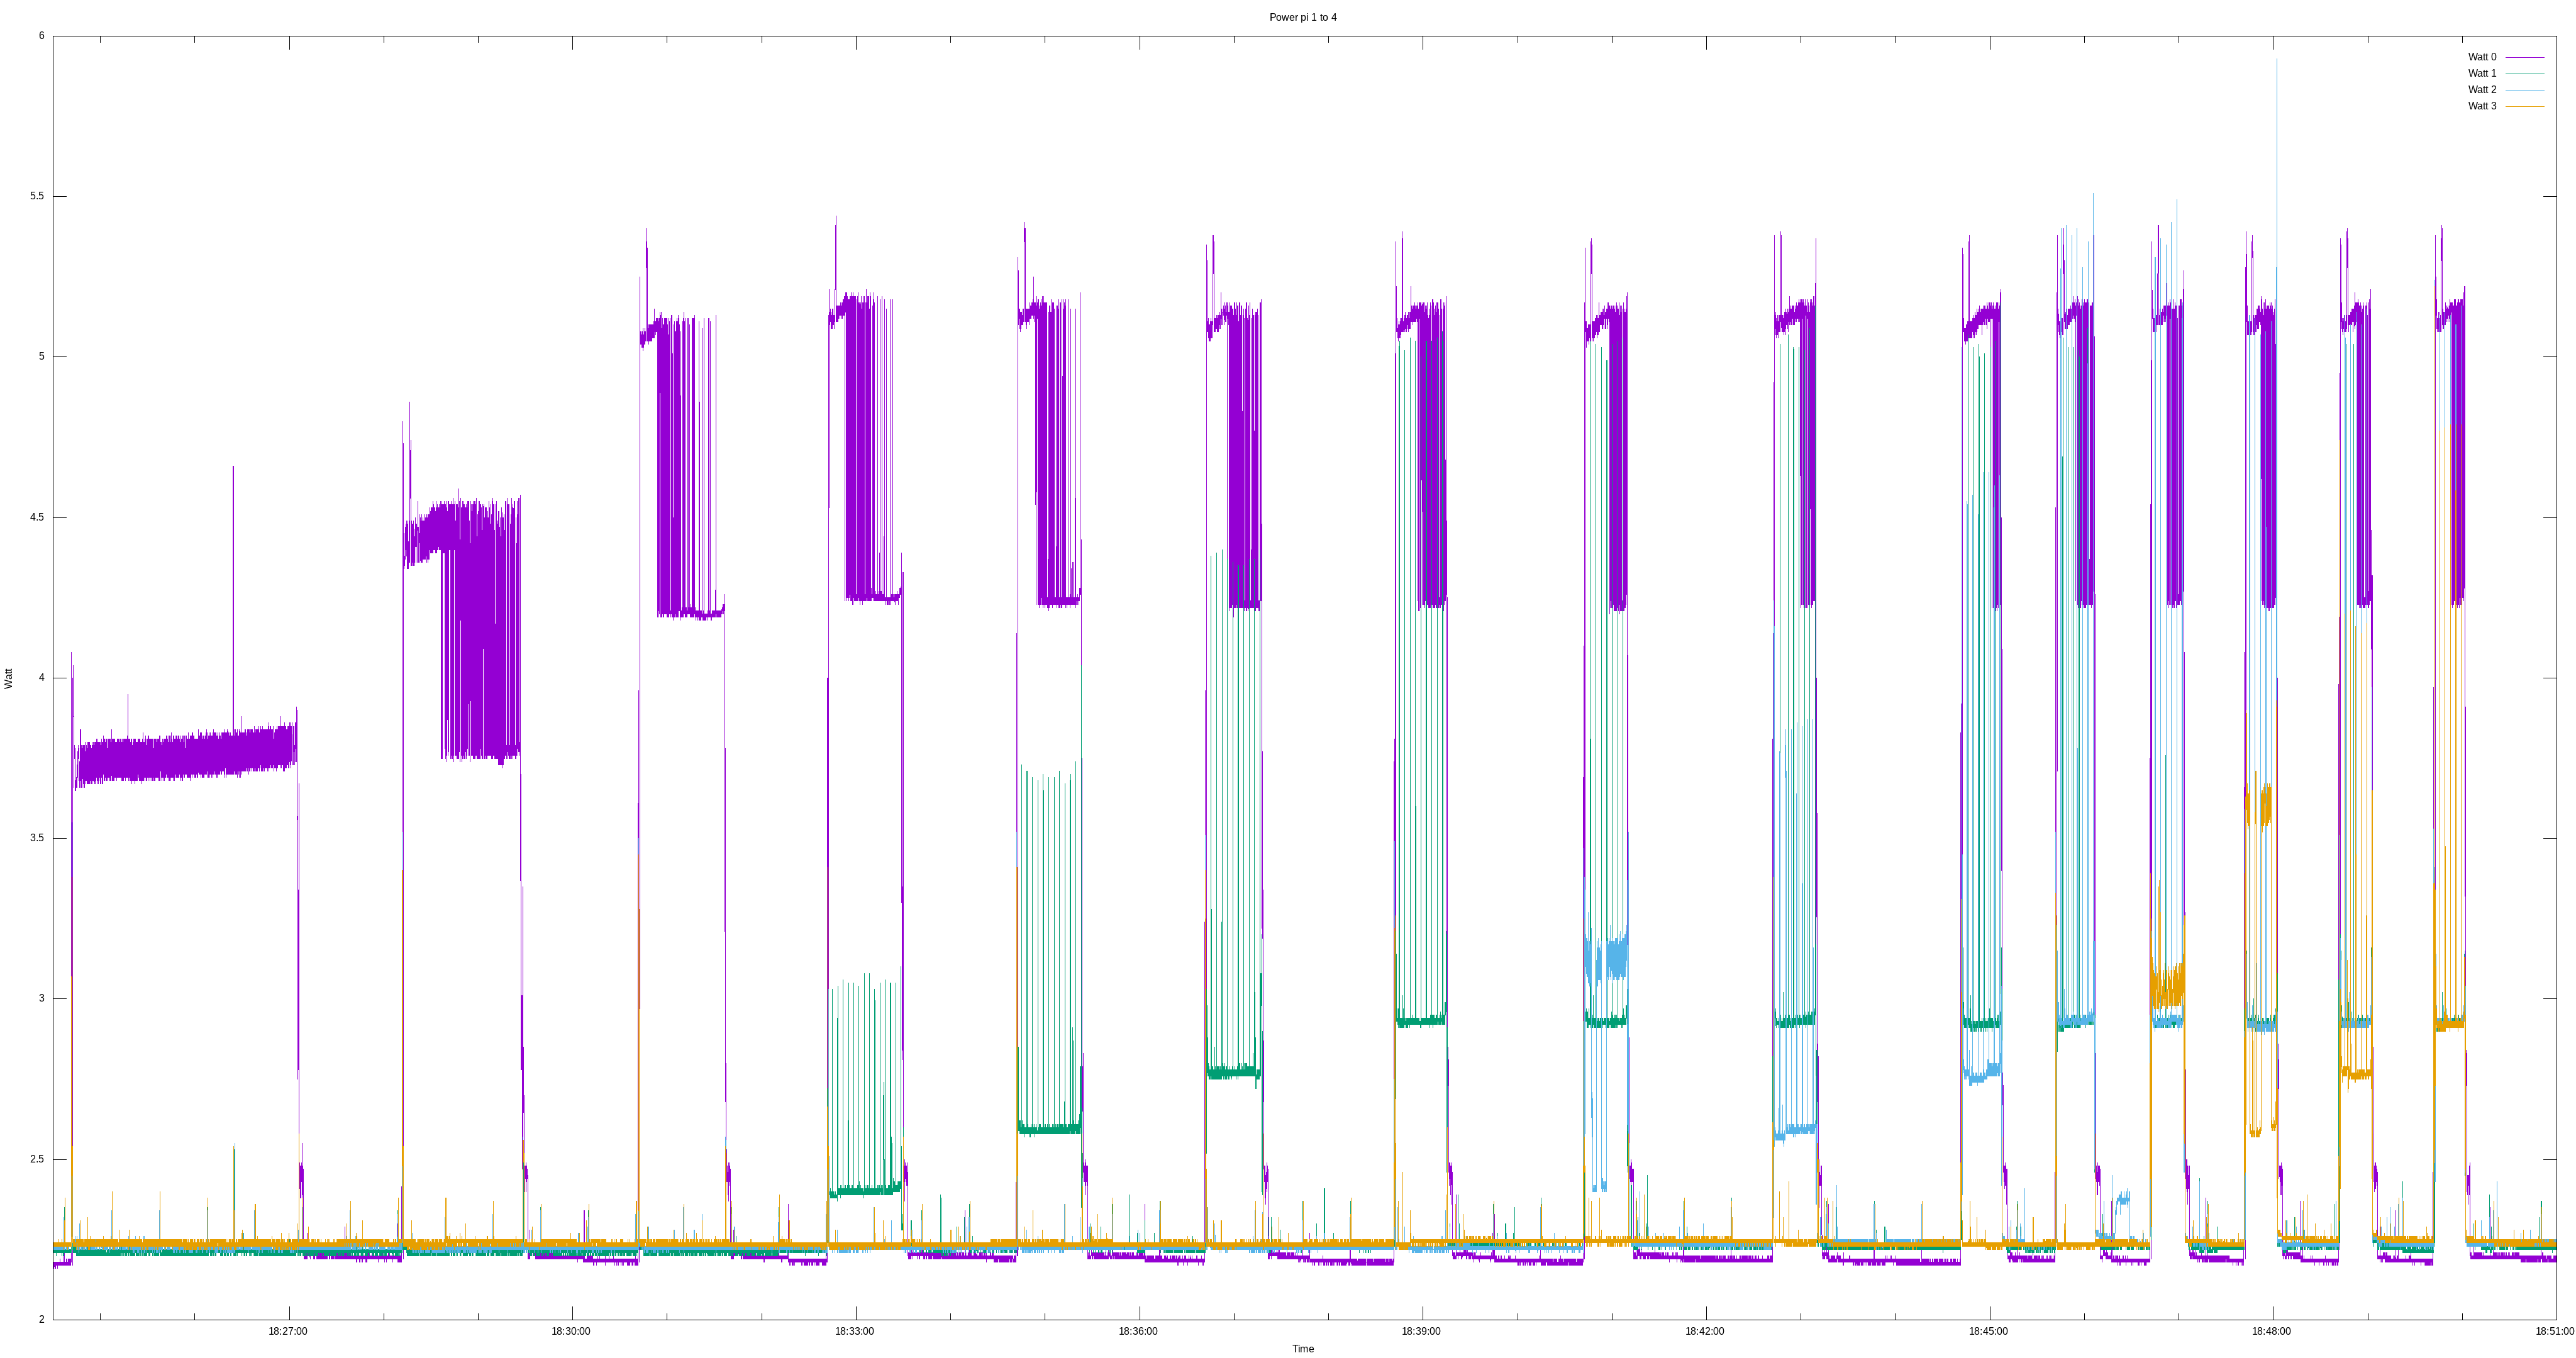
\includegraphics[width=12cm]{images/power.png}
\caption{Power cponsumed during Mandelbrot test}
\label{fig:Mandelgnuplot}
\end{figure}

\begin{figure}[H]
\centering
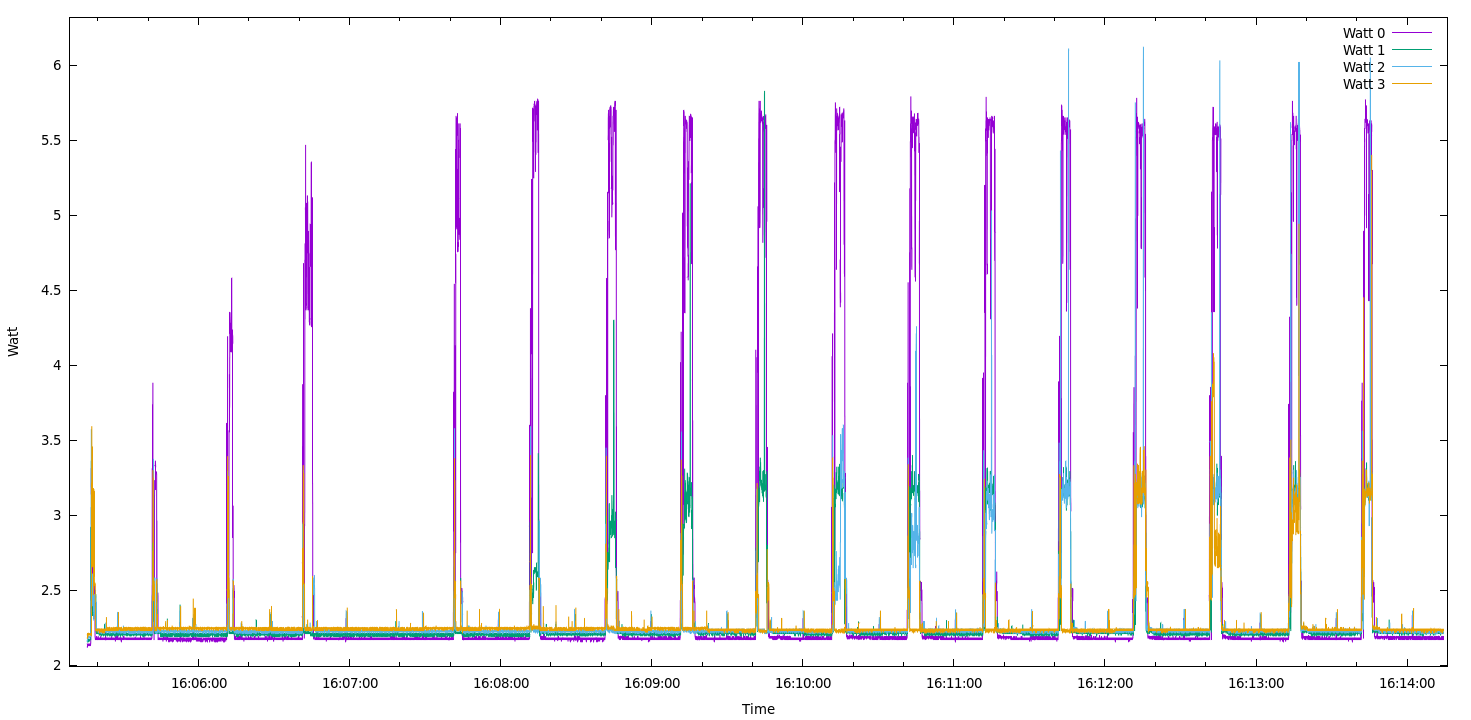
\includegraphics[width=12cm]{images/wattage.png}
\caption{Power consumed during FFT test}
\label{fig:FFTgnuplot}
\end{figure}

Afterwards we calculated the average power used in idle state for all the raspberry pi's. Then the average power used by each raspberry pi during each run. We subtracted the idle value from the runtime value. This was then multiplied with the runtime (in hours) calculated by the program. Which resulted in the graphs seen in figure \ref{fig:Mandelgraph} and \ref{fig:FFTgraph}.

\begin{figure}[H]
\centering
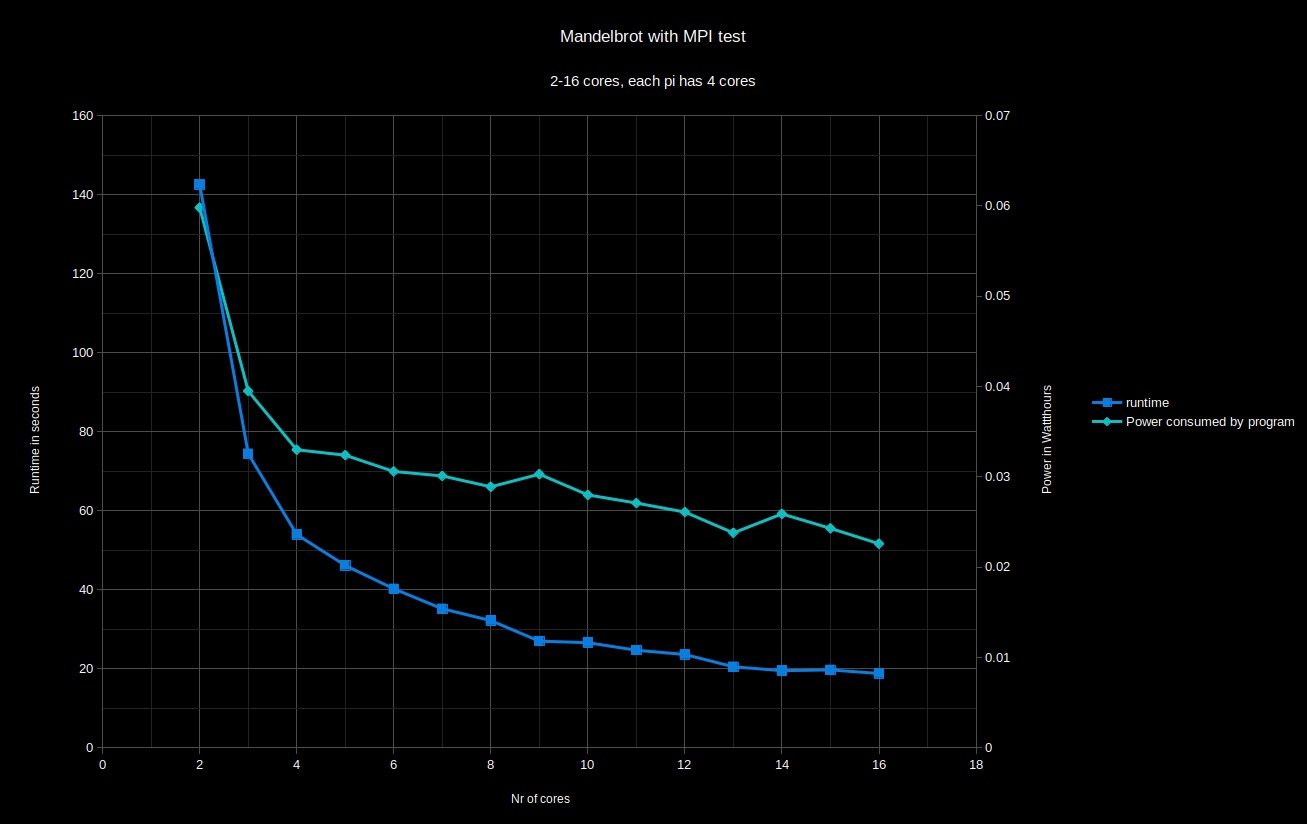
\includegraphics[width=12cm]{images/Mandelbrot.png}
\caption{Compared Runtime vs Power consumed over cores used during Mandelbrot test}
\label{fig:Mandelgraph}
\end{figure}

\begin{figure}[H]
\centering
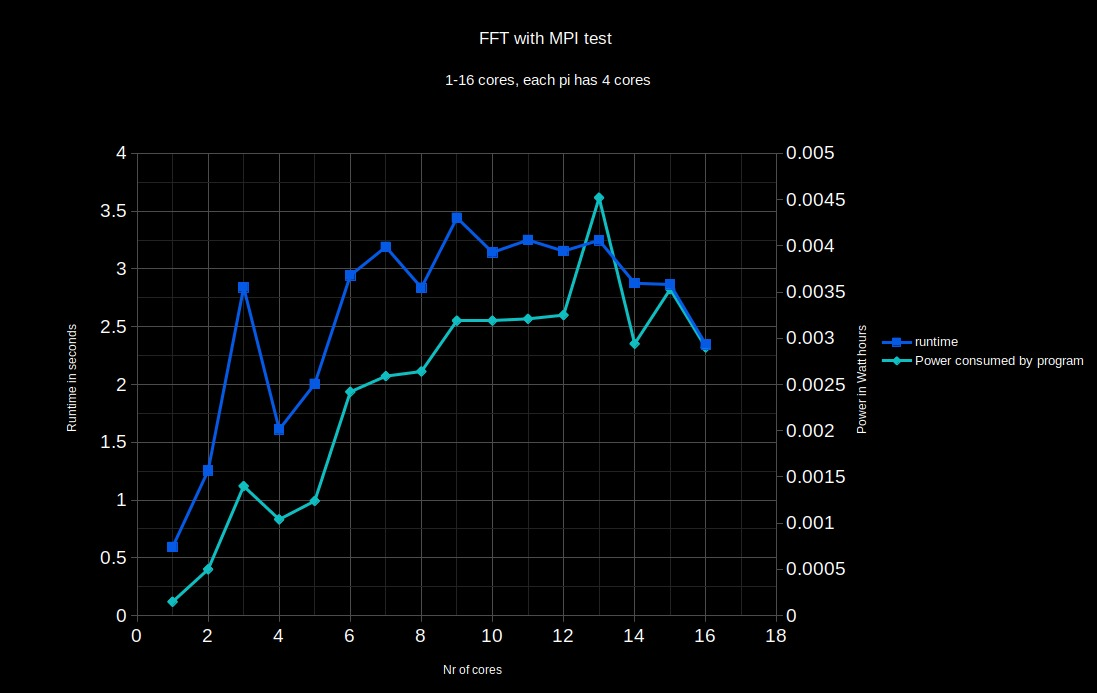
\includegraphics[width=12cm]{images/FFTMPI.png}
\caption{Compared Runtime vs Power consumed over cores used during FFT test}
\label{fig:FFTgraph}
\end{figure}

\section{Discussion}
During testing and analysis we noted some results we found questionable. In figure \ref{fig:dirtymandel} we have the results of a Mandelbrot test before we preformed a clean install. Especially in the idle state the power consumption is fluctuating heavily in comparison with the Mandelbrot test after the clean install, figure \ref{fig:Mandelgnuplot}.  

\begin{figure}[H]
\centering
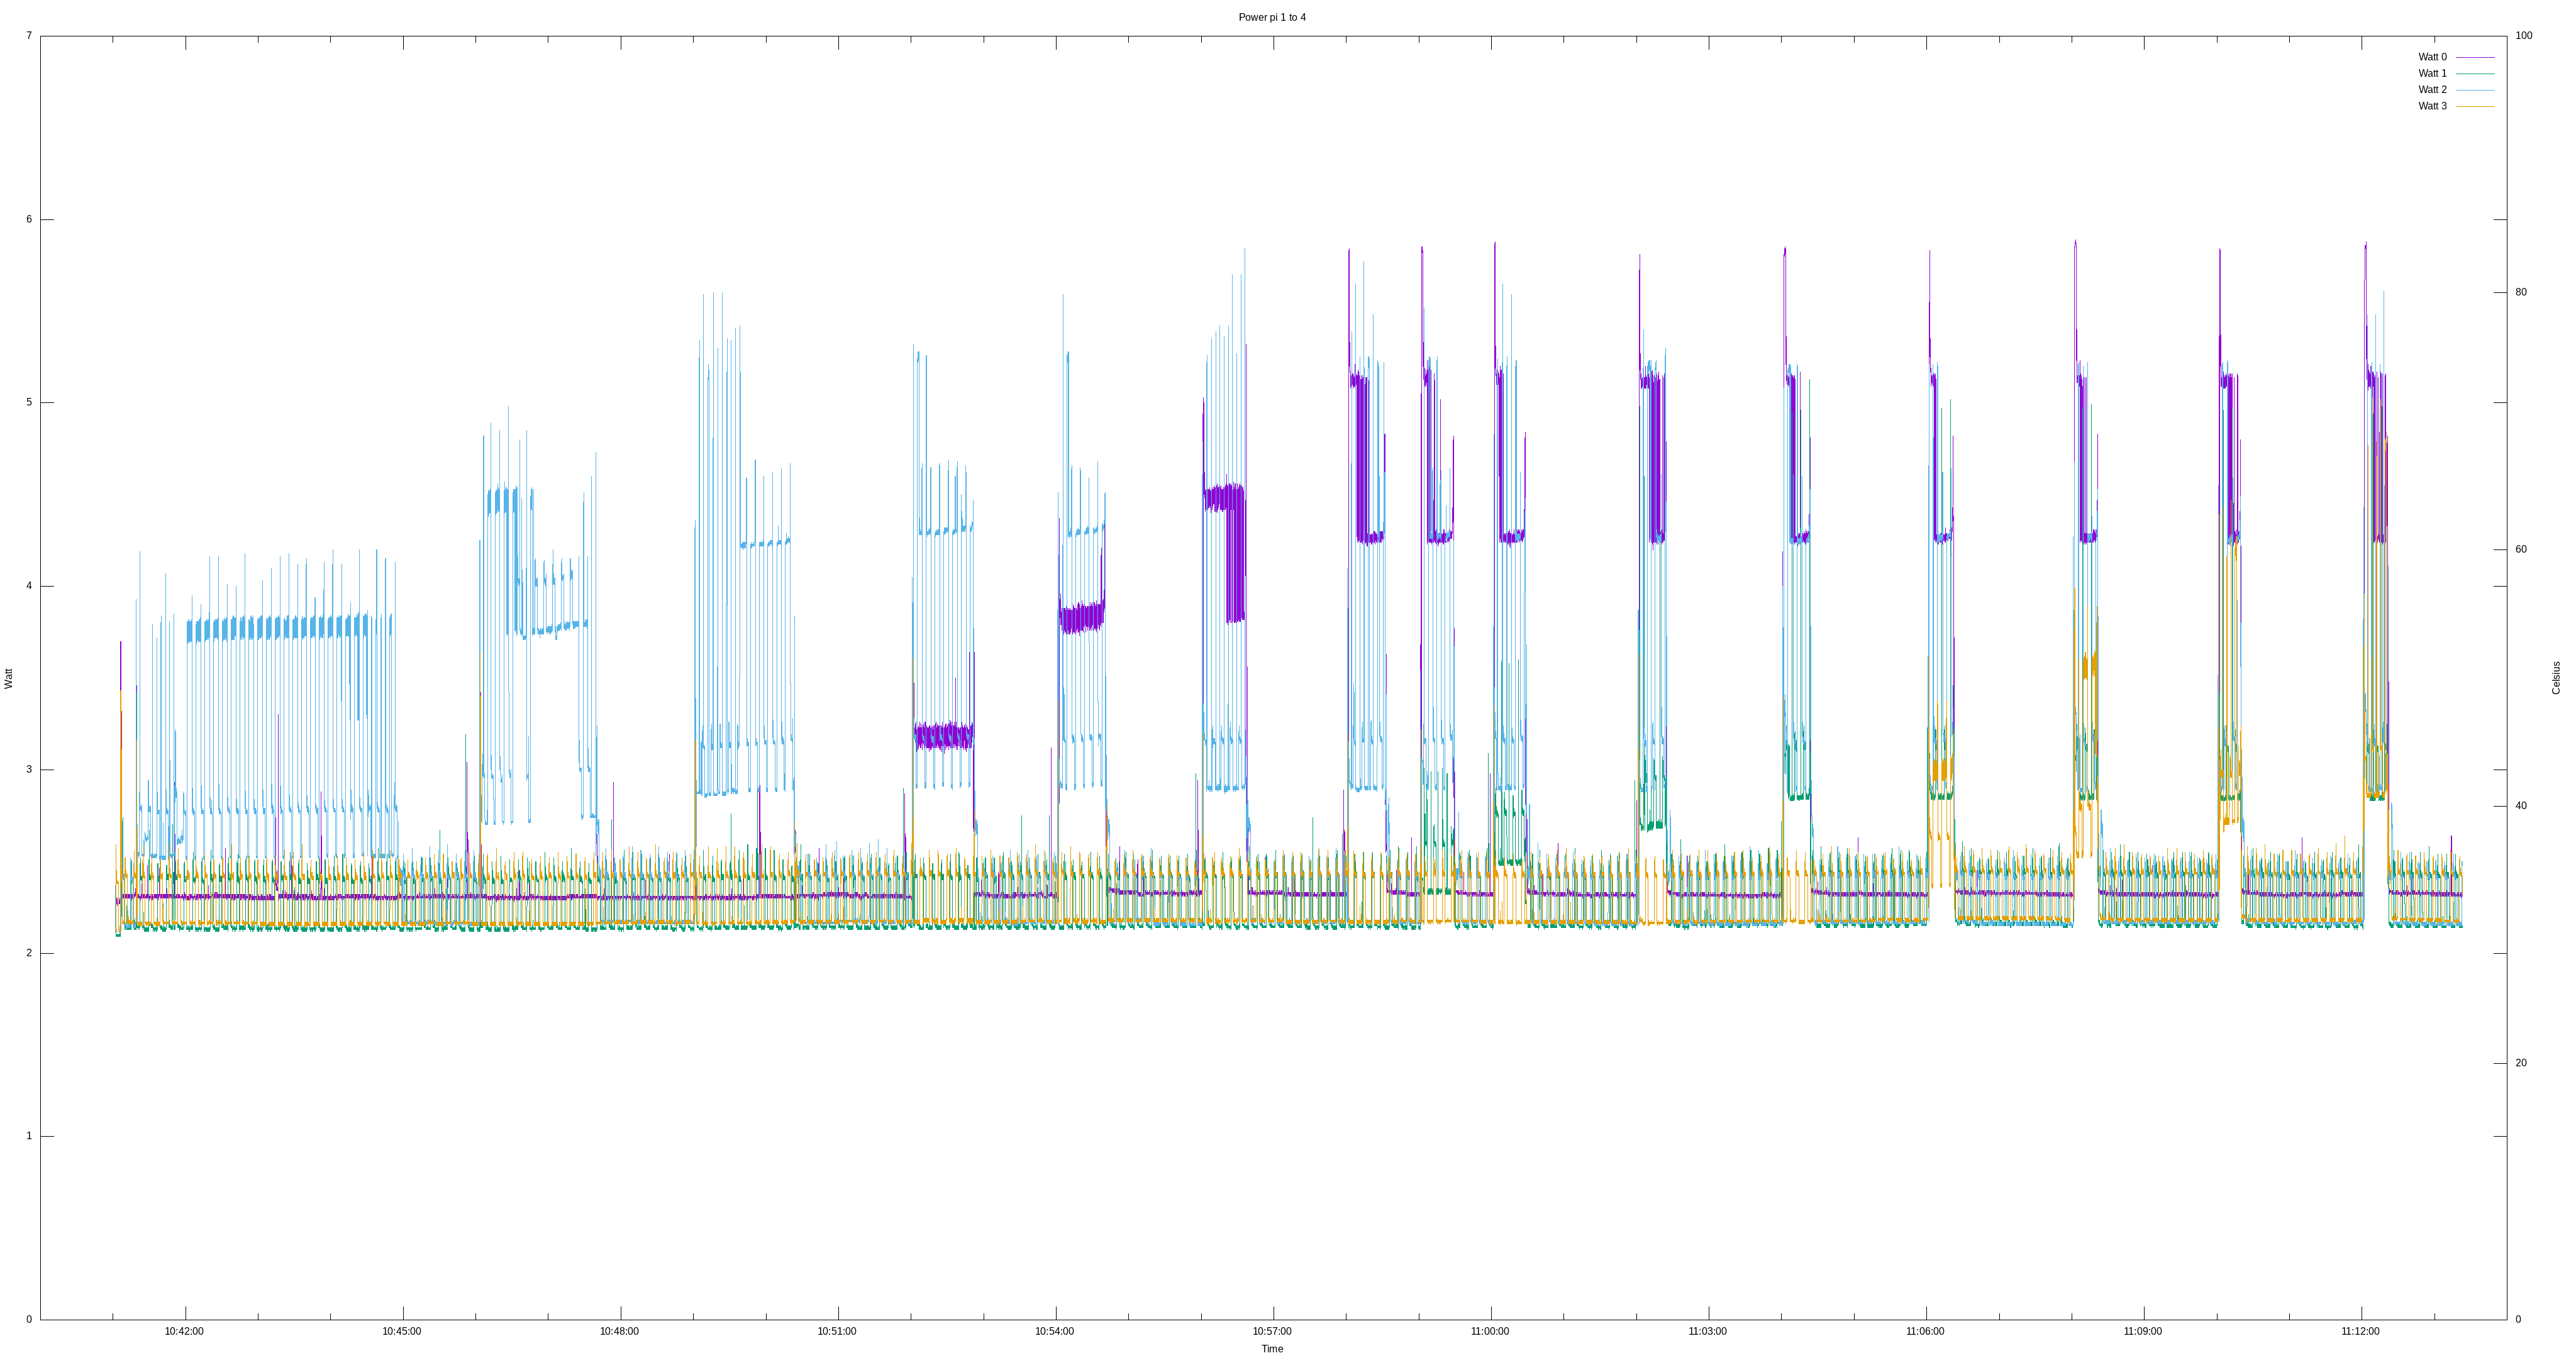
\includegraphics[width=12cm]{images/dirtypower.png}
\caption{Power consumed during Mandelbrot test before clean install}
\label{fig:dirtymandel}
\end{figure}

In the beginning we thought the fluctuation was normal for the raspberry pi as we suspected it had to do with background tasks which needed to be performed. Now we know this most likely had to do with an old installation of Docker which was no longer in use. 
\newline
If we had continued all the tests with this setup our results would not be valid since the process would be disrupted and we would not solely measure the algorithm.\\

Also note in figure \ref{fig:Mandelgraph} that the runtime isn't at it's lowest point yet, this implies that more than 16 raspberrypi cores are needed to get interesting results. In a future setup consider adding more pi's to the stack.\\ 

Some notes on the algorithm:\\

The FFTW with multithreading test can't use any image as input yet.
The FFTW library requires that your input is a one dimensional string. Currently we've created a program that takes the hex values of each pixel of an image and prints that. Then we've put the output in a .hpp file as a one dimensional string. This however limits the max size you can input. \par Ideally we want the program to be able to take any image as input then internally convert this to a one dimensional string and then preform a Fourier transform.\\

.FITS files are the most common file types used in radio astronomy and could be looked into 

Due to the small size of the Fourier transform in the current program the data isn't really use full for representing the big data loads that astronomy super computers endure. It only proves that with small programs the extra communication complicates the program and increases the amount of time it takes to calculate, while also increasing the power consumption.

\section{Conclusion}
After concluding our tests and finishing our analysis we can state that the research is not yet completed. The research and tests that remain are too great to truly answer our research questions at this moment. We are content with our work and our tests have shown the potential of our working setup. Which is what we wanted to achieve to help find the answers we were looking for. The ideas we wrote down in the chapter Future plans are what we see as the starting points for the new teams to bring this research further and come to a true conclusion. 
\end{document}
